\begin{frame}
    \frametitle{Skewness Analysis}
    \begin{itemize}
        \item \textbf{Formulas:}
        \[
        \begin{aligned}
        \text{Moments Skewness} &= \frac{\mu_3}{\sigma^3} \\
        \text{Pearson Skewness} &= \frac{3(\bar{x} - \tilde{x})}{\sigma} \\
        \text{Bowley Skewness} &= \frac{Q_1 + Q_3 - 2\tilde{x}}{Q_3 - Q_1}
        \end{aligned}
        \]
        
        \item \textbf{Results:}
        \begin{itemize}
            \item Moment Coefficient: 0.649
            \item Pearson's Skewness: 0.250
            \item Bowley's Skewness: 0.052
        \end{itemize}
        
        \item \textbf{Interpretation:} Positive skewness across all measures confirms right-tailed distribution. Moderate skewness (0.649) suggests common outliers in higher incidence rates.
    \end{itemize}
\end{frame}

\begin{frame}
    \frametitle{Kurtosis Analysis}
    \begin{itemize}
        \item \textbf{Formula:}
        \[
        \text{Excess Kurtosis} = \frac{\mu_4}{\sigma^4} - 3
        \]
        
        \item \textbf{Result:}
        \begin{itemize}
            \item Excess Kurtosis: 0.241
        \end{itemize}
        
        \item \textbf{Interpretation:} Positive value indicates leptokurtic distribution (sharper peak than normal), suggesting clustering around mean with heavy tails of extreme values.
    \end{itemize}
\end{frame}

\begin{frame}
    \frametitle{Skewness Measures Comparison}
    \centering
    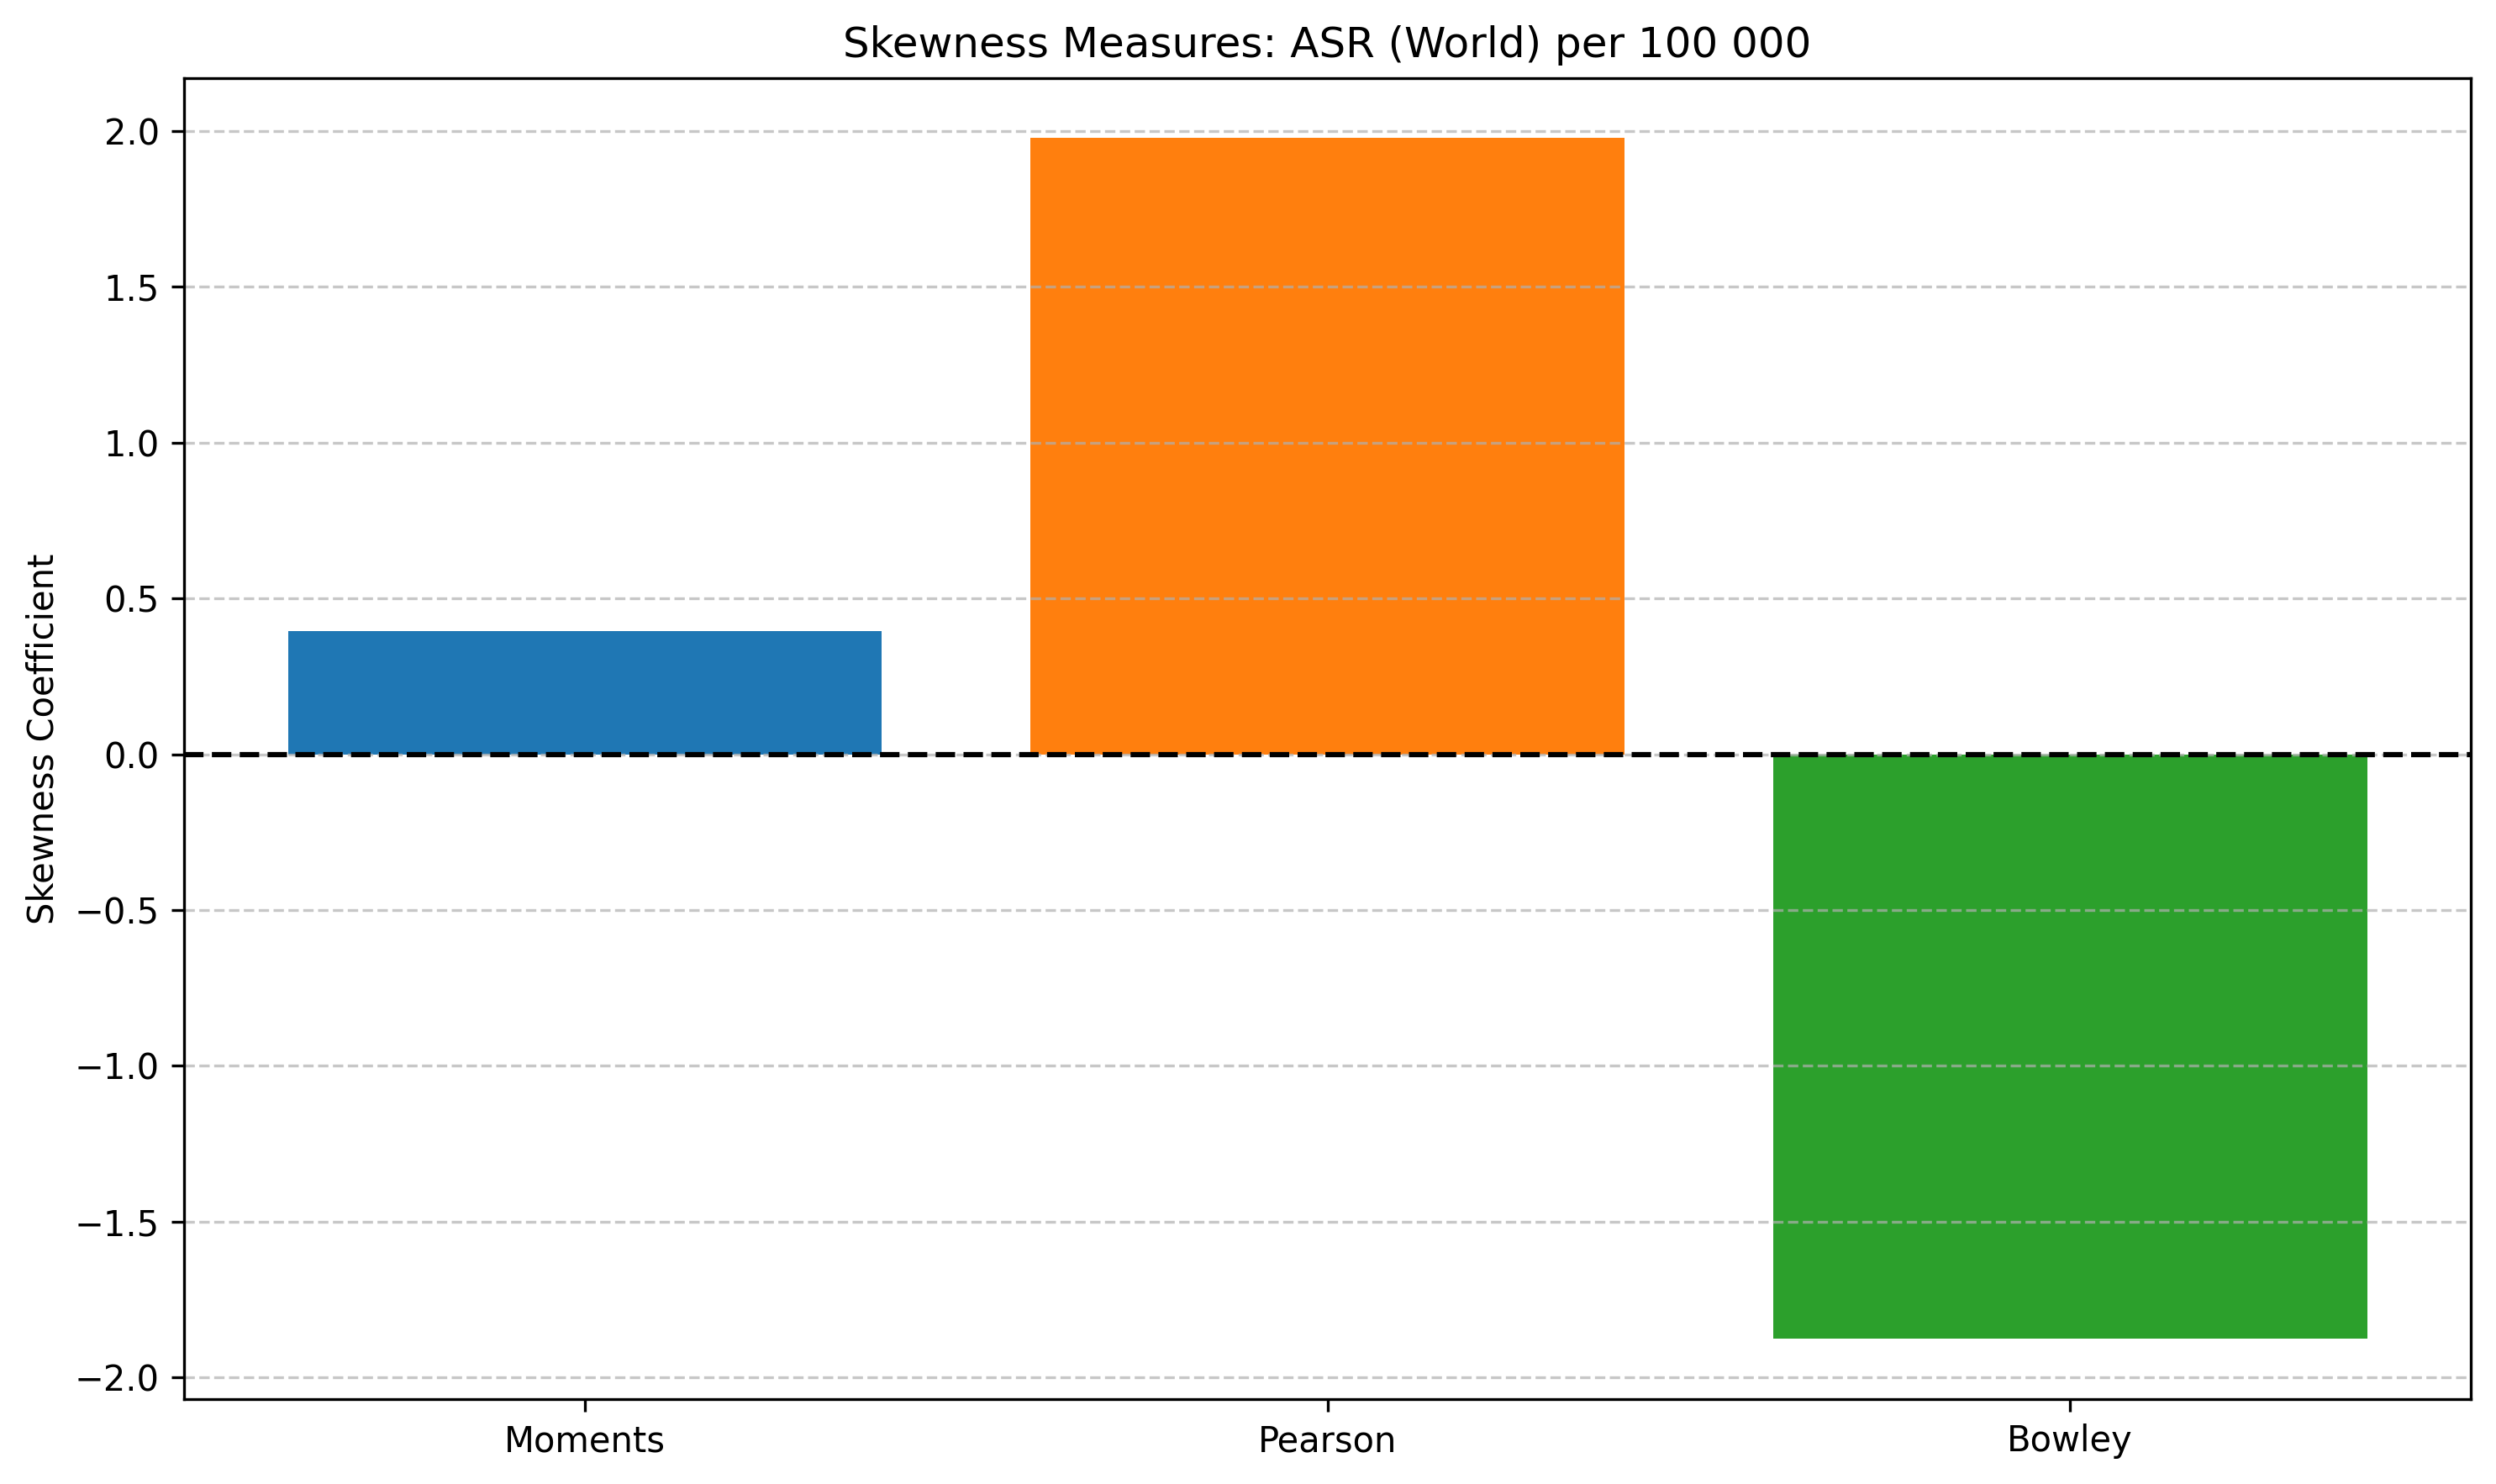
\includegraphics[width=0.75\textwidth,height=0.6\textheight,keepaspectratio]{images/graph/skewness_comparison.png}
    \vspace{-0.5em}
    \begin{itemize}
        \item \textbf{Key Observation:}
        \begin{itemize}
            \item Moment measure most sensitive to outliers
            \item Bowley's measure shows mild asymmetry in middle 50\% data
            \item All measures agree on positive direction of skew
        \end{itemize}
    \end{itemize}
\end{frame}